Os mercados normalmente definem uma quantidade mínima por lote ofertado. Se uma bolsa determina um mínimo de 100 ações um vendedor não poderia criar uma oferta de 50 ações. Se os preços ofertados no momento permitirem a execução de um negócio, a transação ocorrerá em cima da menor quantidade entre as duas ofertas, ou seja, se uma ordem de venda de 100 ações fecha um negócio com uma ordem de compra de 200 ações por exemplo, a quantidade negociada será de apenas 100. O restante da oferta de compra, i.e. 100 ações, continua no livro de oferta de compras, enquanto no lado da venda, a próxima oferta de maior preferência vai para o topo do livro. 

Definimos como $p^{a}$ o preço de uma determinada oferta de venda, chamado de \textit{ask} em inglês e $p^{b}$ para compras, ou \textit{bid} em inglês. Um agente pode ter diversas ofertas para cada ativo $i$, em tempos diferentes indexados pelo símbolo $t$: 
\begin{equation*}
	\begin{aligned}
		p^{a}_{t, i} \text{ para ofertas de venda e}  \\
		p^{b}_{t, i} \text{ para ofertas de compra.}
	\end{aligned}
\end{equation*}

A posição de uma oferta no livro de vendas para um ativo $i$ é dada pela função $\mathbf{pos}_{t, i}^{a}(p) = k$ está na posição $k$ da fila \footnote{onde $k = 0$ é a melhor oferta; com valores de preço decrescentes para vendas, e crescentes para compras.}. A diferença entre ofertas de compra e venda para um mesmo ativo $\Delta_{t, i} = p_{t, i}^{a} - p_{t, i}^{b}$ é o \textit{spread} no momento $t$ e caso $\mathbf{pos}_{t, i}^{a}(p) = \mathbf{pos}_{t, i}^{b}(p) = 0$ é chamado de \textit{bid-ask spread} $\mathbf{\Delta}_{t, i}$.

O objetivo de uma estratégia de \textit{market making} (\textit{MM}) nesse contexto é criar ofertas de compra com valor maior que a melhor oferta, ou menor para ofertas de venda que venham a se tornar as melhores ofertas:

\begin{itemize}
    \item de venda, tais que $p^{a} < P^{a}$; ou 
    \item de compra, tais que $p^{b} > P^{b,}$;
\end{itemize}

onde $p$ é o preço da oferta do agente e $P$ é a melhor oferta existente $\mathbf{pos}_{t, i}^{a}(P) = \mathbf{pos}_{t, i}^{b}(P) = 0$.
É importante notar que quaisquer ordens criadas por um agente de \textit{MM} não geram novas transações no instante \textit{t} (indicado por $p^{a} > P^{b}$ e $p^{b} < P^{a}$ para um mesmo ativo). A seguir um exemplo da reta de preços para um momento $t$ e um ativo $i$ qualquer, onde $p^{b, k}$ é tal que $\mathbf{pos}^{b}(p^{b, k}) = k$:

\begin{figure}
	\begin{center}
		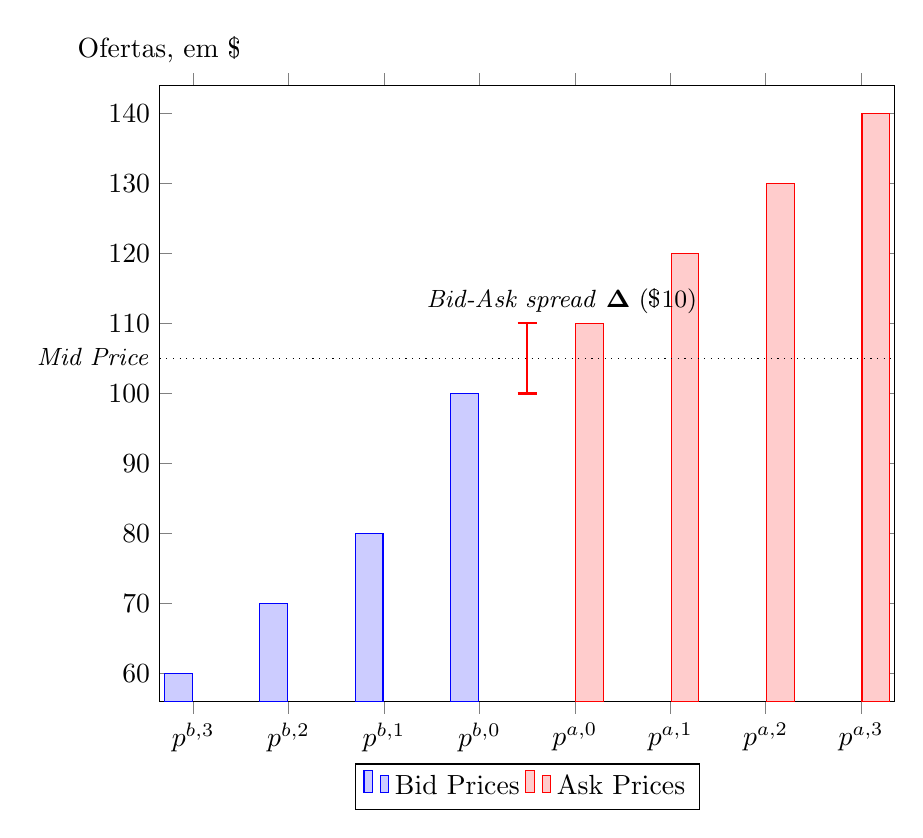
\begin{tikzpicture}
			\begin{axis}[
				x tick label style={/pgf/number format/1000 sep=},
				enlargelimits=0.05,
				legend style={at={(0.5,-0.1)}, anchor=north,legend columns=-1},
				ybar=0.7,
				ylabel={Ofertas, em \$},
    				ylabel style={
    				at={(0,1.02)},
    				anchor=south,
    				rotate=-90,
    			},
				width=0.9\textwidth, % Adjust the width to fit within the box
				xticklabels={
					$p^{b, 3}$, $p^{b, 2}$, $p^{b, 1}$, $p^{b, 0}$, 
					$p^{a, 0}$, $p^{a, 1}$, $p^{a, 2}$, $p^{a, 3}$
					},
				xtick={1,2,3,4,5,6,7,8}, % Set explicit tick positions
				after end axis/.code={
					\draw [red, thick, line cap=] (axis cs:4.5,100) -- (axis cs:4.5,110); % Static vertical line for spread with end caps
					\draw [red, thick] (axis cs:4.4,100) -- (axis cs:4.6,100);
					\draw [red, thick] (axis cs:4.4,110) -- (axis cs:4.6,110);
					\draw [black, dotted] (axis cs:0.65,105) -- (axis cs:8.35,105);
					\node[right, font=\small] at (rel axis cs:0.35,0.65) {\textit{Bid-Ask spread} $\mathbf{\Delta}$ (\$10)}; % Label for the spread line
					\node[left, font=\small] at (rel axis cs:0,0.56) {\textit{Mid Price}};
				}
				]
				% Represent bid prices in blue
				\addplot [blue, fill=blue!20] coordinates {(1, 60) (2, 70) (3, 80) (4, 100)};
				% Represent ask prices in red
				\addplot [red, fill=red!20] coordinates {(5, 110) (6, 120) (7, 130) (8, 140)};
				\legend{Bid Prices, Ask Prices}
			\end{axis}
		\end{tikzpicture}
	\end{center}
	\caption{Gráfico de ofertas de um livro de ordens limite $L$ qualquer}
\end{figure}

\begin{figure}
	\begin{center}
		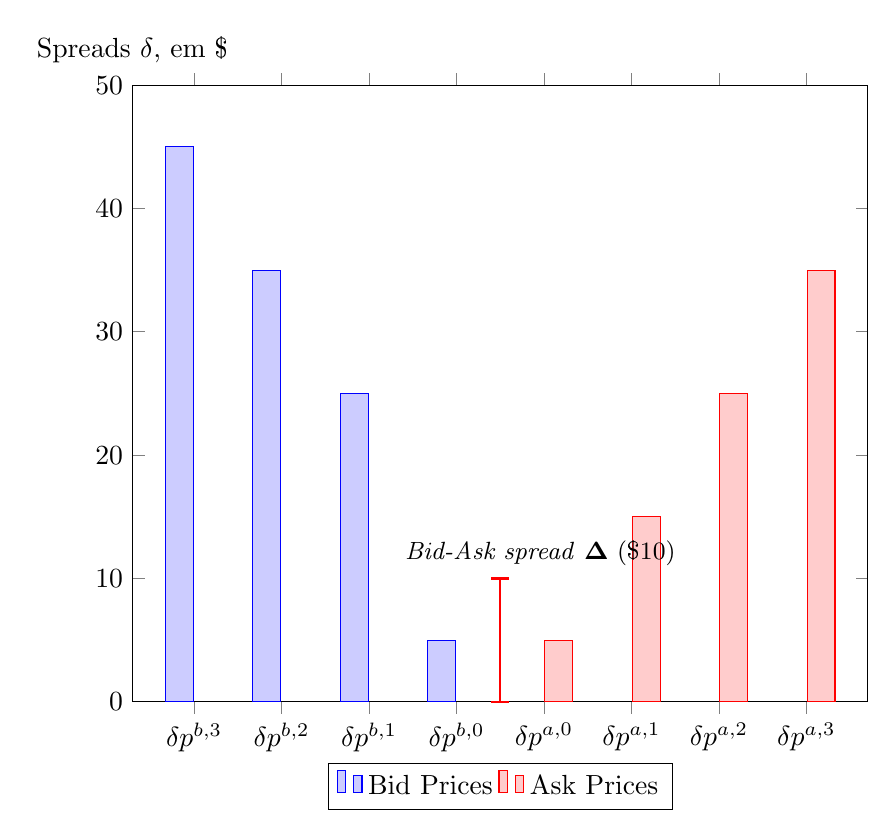
\begin{tikzpicture}
			\begin{axis}[
				x tick label style={/pgf/number format/1000 sep=},
				legend style={at={(0.5,-0.1)}, anchor=north,legend columns=-1},
				ybar=0.7,
				ylabel={Spreads $\delta$, em \$},
				ylabel style={
					at={(0,1.02)},
					anchor=south,
					rotate=-90,
				},
				ymin=0, ymax=50,
				width=0.9\textwidth, % Adjust the width to fit within the box
				xticklabels={
					$\delta p^{b, 3}$, $\delta p^{b, 2}$, $\delta p^{b, 1}$, $\delta p^{b, 0}$, 
					$\delta p^{a, 0}$, $\delta p^{a, 1}$, $\delta p^{a, 2}$, $\delta p^{a, 3}$
					},
				xtick={1,2,3,4,5,6,7,8}, % Set explicit tick positions
				after end axis/.code={
					\draw [red, thick, line cap=] (axis cs:4.5,0) -- (axis cs:4.5,10); 
					% Static vertical line for spread with end caps
					\draw [red, thick] (axis cs:4.4,0) -- (axis cs:4.6,0);
					\draw [red, thick] (axis cs:4.4,10) -- (axis cs:4.6,10);
					\node[right, font=\small] at (axis cs:3.3,12) {\textit{Bid-Ask spread} $\mathbf{\Delta}$ (\$10)}; % Label for the spread line
				}
				]
				% Represent bid prices in blue
				\addplot [blue, fill=blue!20] coordinates {(1, 45) (2, 35) (3, 25) (4, 5)};
				% Represent ask prices in red
				\addplot [red, fill=red!20] coordinates {(5, 5) (6, 15) (7, 25) (8, 35)};
				\legend{Bid Prices, Ask Prices}
			\end{axis}
		\end{tikzpicture}
	\end{center}
	\caption{Gráfico de spreads de um livro de ordens limite $L$ qualquer}
\end{figure}

Para ilustrar melhor o funcionamento do livro de ordens considere a seguinte situação para um mesmo momento e ativo: um agente qualquer de \textit{MM} tem a \textbf{única oferta de venda} pelo preço de $p^{a}$ no mercado. Caso surja uma nova oferta de \textbf{compra} com melhor preço e acima do preço da oferta do agente $P^{b} \geq p^{a}$, será gerada uma transação pelo preço $p^{a}$ e a ordem de preço $P^{b}$ que gerou a transação é chamada de ordem de mercado, enquanto a ordem do agente é chamada de ordem limite. Após o motor de transações da bolsa receber a ordem com preço $P$, uma transação ocorre e ambas ofertas são removidas do livro de ordens. Em seguida, o agente tem sua posição $r_{t}$ ajustada:
\begin{equation}
    \begin{aligned}
    	r_{t + 1}:= r_{t} + p^{a}q \text{ para vendas e} \\ 
    	r_{t + 1}:= r_{t} - p^{b}q \text{ para compras}
    \end{aligned}
\end{equation}
sendo $r_{t}$ o valor da posição do agente no instante $t$ e $q$ a quantidade de ativos negociadas na transação em questão.

O agente em seguida escolhe esperar ou realizar uma das ações abaixo:
\begin{enumerate}
    \item inserir uma nova oferta de venda, substituindo a oferta anterior;
    \item inserir ou ajustar uma oferta de compra existente no livro de ofertas de compras;
\end{enumerate}

A decisão do agente irá depender de sua expectativa sobre a evolução do mercado, assim como do processo de chegada de ordens de outros agentes, representados pelo identificador $n$, incluindo, mas não limitado à
\begin{itemize}
    \item probabilidade de chegar uma oferta de compra com preço superior $Pr(P_{t + s, i}^{b} > p_{t, i}^{b})$, em algum momento no futuro $s > 0$;
    \item probabilidade de chegar uma oferta de venda com preço inferior $Pr(P_{t + s, i}^{a} < p_{t, i}^{a})$, em algum momento no futuro $s > 0$;
    \item liquidez esperada para o mercado a partir de $t$ até o momento de fechamento do pregão $T$;
    \item risco futuro da posição ultrapassar os limites estabelecidos pelas corretoras.
\end{itemize}

De modo a simplificar as equações adiantes e utilizar uma notação mais comumente usada no contexto de ordens limite, definimos:

\begin{description}[]
	\item[$\delta_{t}(p)$:] $\mathbb{R} \rightarrow \mathbb{R} = |p - p_{t}|$ como a diferença entre o preço $p$ de uma oferta de venda ou compra e o preço de mercado $p$ da ação subjacente no momento $t$.
	
	\item[$\delta_{t}(p, q)$:] $\mathbb{R}^{2} \rightarrow \mathbb{R} = q \cdot \delta_{t}(p)$ como a função que mapeia o impacto de $q$ ações negociadas na carteira do agente sob o \textit{spread} parcial $\delta_t$.
	
	\item[$r_{t}$] é o retorno obtido pelo agente no momento $t$. É calculado pela soma do impacto de todos ativos, onde $o_{t} = \{(p_{t, 0}^{a}, Q_{t, 0}^{a}), ..., (p_{t, n}^{a}, Q_{t, n}^{a}), (p_{t, 0}^{b}, Q_{t, 0}^{b}), ..., (p_{t, m}^{b}, Q_{t, m}^{b})\}$ é o conjunto de ofertas do agente para todos ativos no momento $t$. Cada oferta é uma tupla $(p, Q)$ de preço por ativo e quantidade de ativos ofertada.
	
	\begin{equation} \label{return}
		\begin{aligned}
			r_{t} = \sum_{i = 0}^{n} \delta_{t}(p_{t, i}^{a}, q_{t, i}^{a}) \\
			-\sum_{i = 0}^{m} \delta_{t}(p_{t, i}^{b}, q_{t, i}^{b}) \\
			\forall t < T
		\end{aligned}
	\end{equation}
\end{description}

Onde os valores de  $q$ são as quantidades efetivamente executadas da ordem, podendo ser menor (no caso de uma ordem parcial) ou igual à $Q$ (ordem total), onde $Q$ é a quantidade inicialmente ofertada pelo agente.
Para considerar custos de transação — que incluem tipicamente custos da corretora e emolumentos das bolsas — basta alterar a expressão para $r_{t} := r_{t} - c$, sendo $c$ o custo total de todas transações realizadas.

O agente de \textit{MM}, por fim, observa a sua posição acumulada durante todo o período de negociação $T$ para decidir se obteve retorno positivo ou negativo:
\begin{equation} \label{return_accumulated}
    R_{T} = \sum_{t=0}^{T} r_t
\end{equation}
Define-se matematicamente o valor da posição $R_T$ como a agregação das receitas de vendas, e dos custos de compra e de transações até o momento $T$. 
